\section{Data}

This study can be conducted in countries that have a census of health facilities included in the Service Provision Assessment and a corresponding Demographic \& Health Survey. Malawi and Haiti meet this criteria. The first version of the paper was based on Haiti.

\section{DHS geomasking}

\subsection{Displacement Procedure}
\label{subsubsec:dispProc}

The displacement procedure is shown in Figure \ref{fig:displaceProc}. First a random angle is selected, then a random distance up to a limit depending on the community type. Urban communities are displaced up to 2km, rural are displaced up to 5km with a 1\% chance of being displaced up to 10km. If a community is displaced point outside of its original administrative boundary, then the displacement procedure is \textbf{repeated} for that community.

    \begin{figure}[htbp]
        \centering
        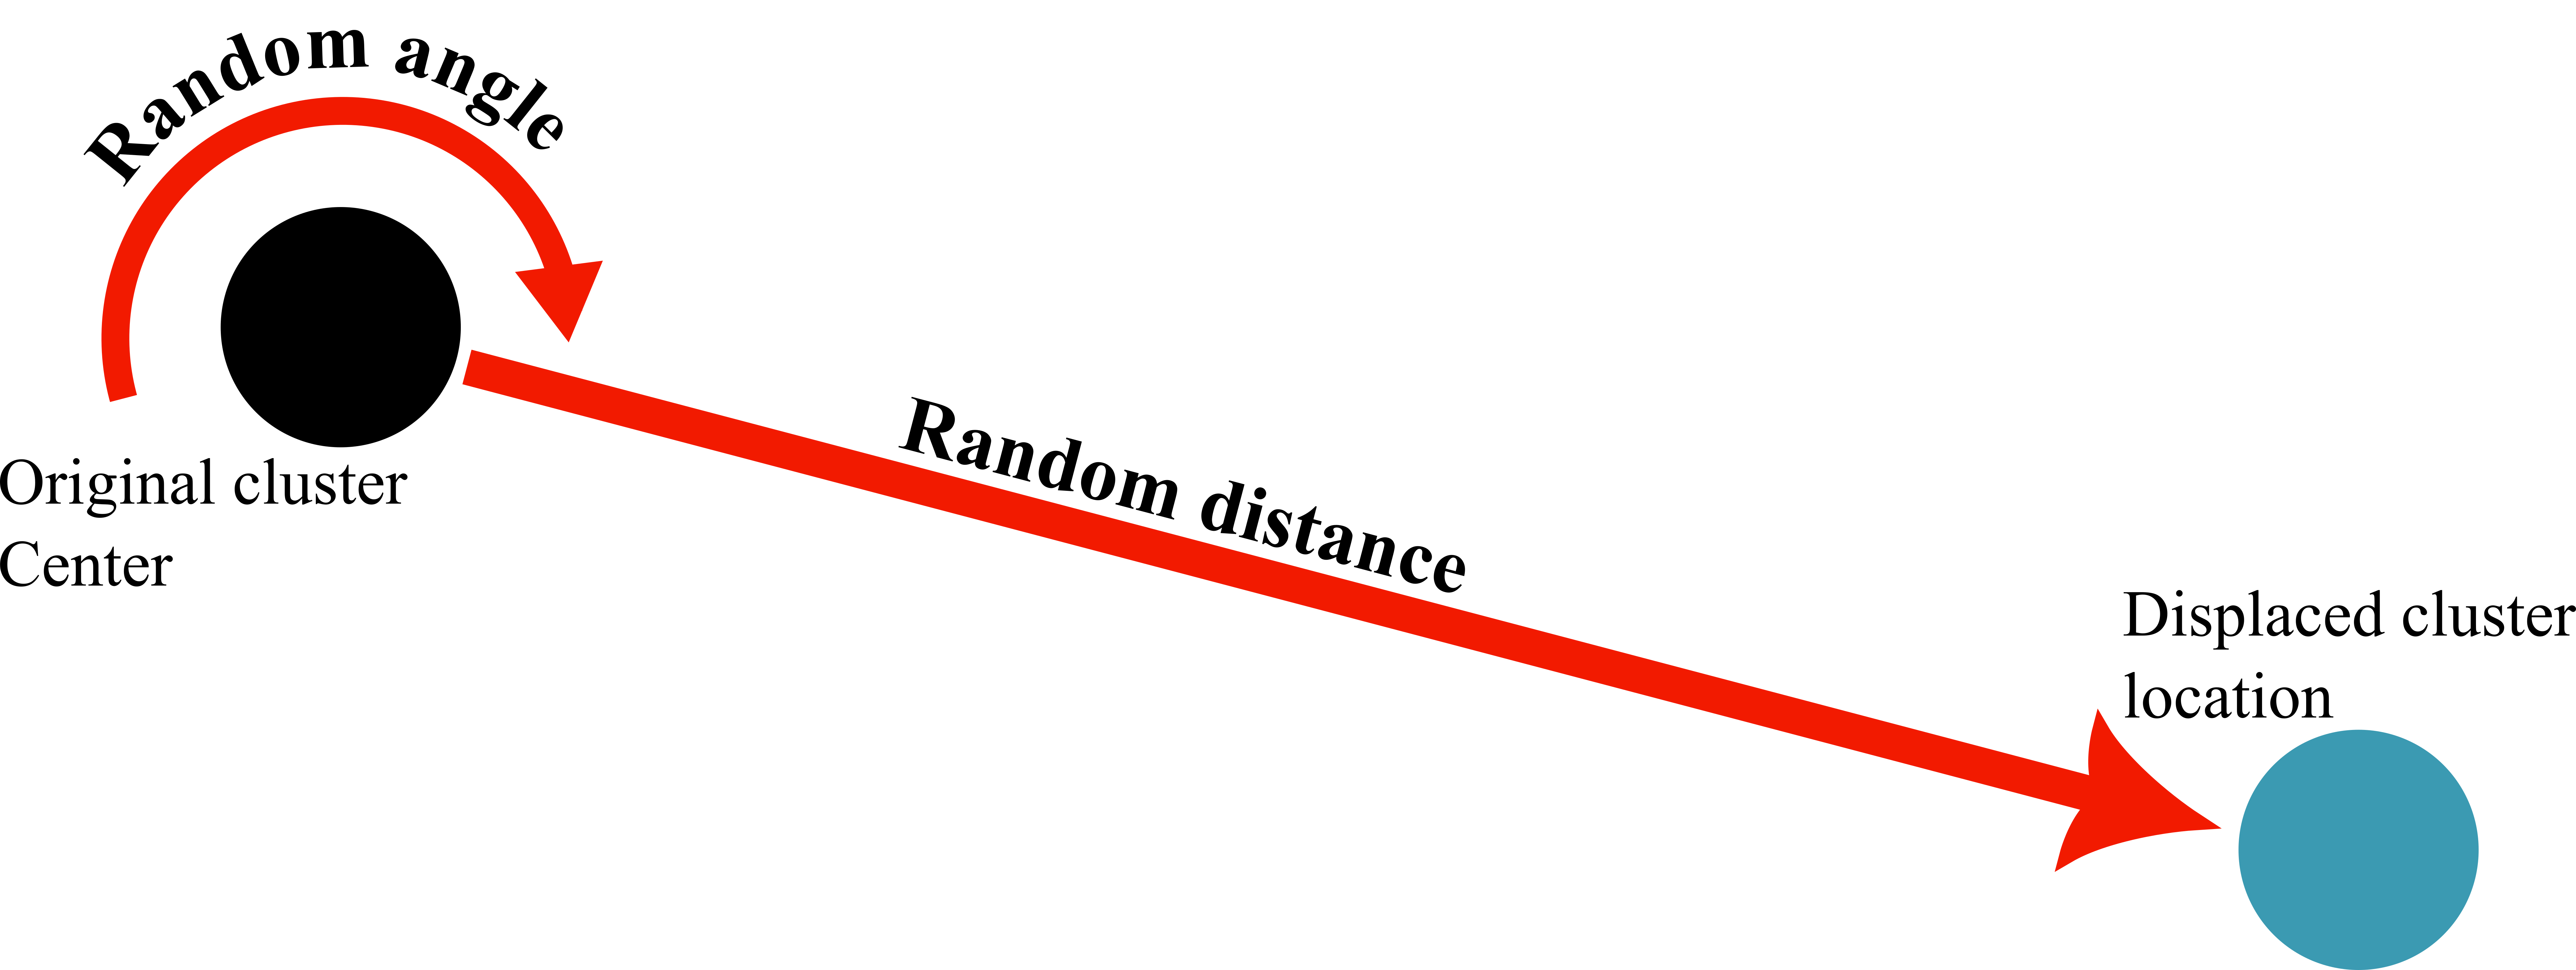
\includegraphics[width=4in]{images/displacement.png}
        \caption{DHS community / cluster displacement procedure \cite{burgert_geographic_2013}}
        \label{fig:displaceProc}
    \end{figure}    

The displacement procedure can be used to define a probability density function (PDF). Equation \ref{eq:pdf} expresses the PDF where $r$ is the limit of the radius of displacement (e.g. 2km for urban communities), and $(x_{0},y_{0})$ are the latitude and longitude distance from the 'true' community location.

\subsection{Probability density function}

    \begin{equation}
    \label{eq:pdf}
f(x_{0},y_{0}) = 
\begin{dcases}
\frac{1}{2\pi r\sqrt{x_{0}^{2}+y_{0}^{2}}}, & \text{if } \sqrt{x_{0}^2 + y_{0}^2} \leq r \\
0, & \text{otherwise}
\end{dcases}
\end{equation}

Alternatively, the symmetry of the PDF can be visualized in Figure \ref{fig:pdf_surface}. An integral of the surface shown in Figure \ref{fig:pdf_surface} gives the probability that the displaced point will fall in a defined area given the true location. Because the PDF is symmetric, integrals of the same PDF can be can be used to calculate the probability of the true location falling in a defined area given the displaced location.

    \begin{figure}[htbp]
        \centering
        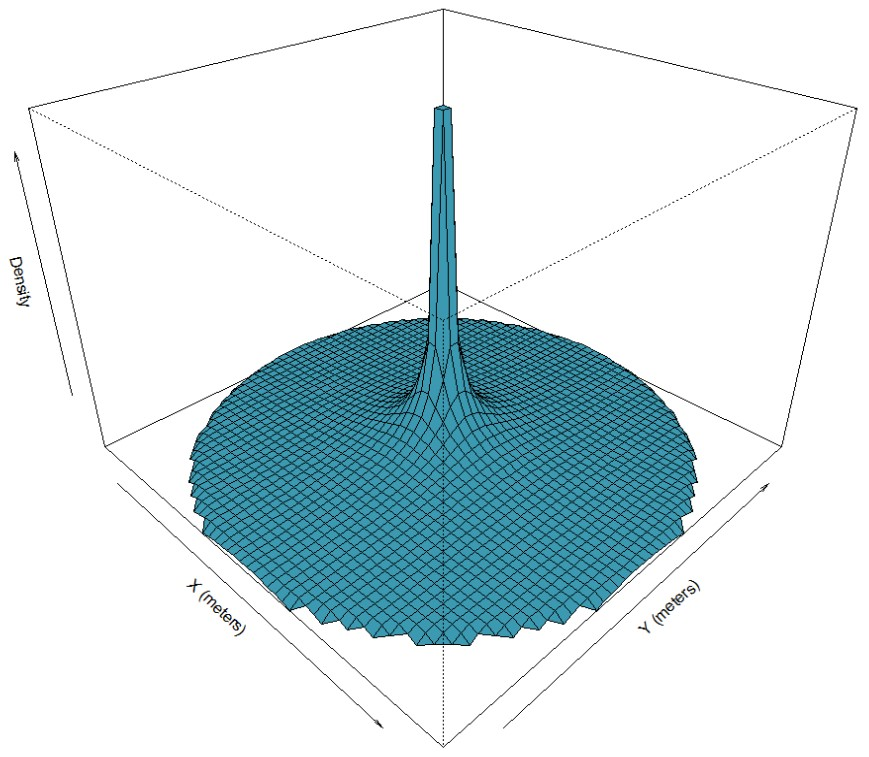
\includegraphics[width=4in]{images/DensityPlot.jpg}
        \caption{Visualization of the surface created by equation \ref{eq:pdf}, with displacement up to $r$ kilometers}
        \label{fig:pdf_surface}
    \end{figure}

Impossible locations (such as those falling outside an administrative boundary) can be trimmed from the probability buffer and the buffer re-weighted so that the volume under the surface sums to one. This buffer can be calculated for a raster at a given resolution, where the layer values are the calculated probabilities that the true cluster center falls within that cell.

To join using the probabilistic approach, a probability raster can be calculated for each displaced community location. A join can be made at the center point of each cell $(x,y)$, and the result of each join at cell $(x,y)$ can be weighted by the probability that the true community location is contained in that cell. An analyst may take a \textbf{}{probability-weighted average} for joining displaced communities to a raster with continuous values. If joining communities to a polygon (such as the catchment area of a health facility), an analyst could use this method to select the \textbf{maximum likely polygon} that a community falls in.

\section{Simulation Study}

I evaluate the performance of the join to a raster created in AccessMod 5.0 \autocite{who_accessmod_2021}, where cell values were travel time in minutes to the nearest health facility from the 2018 SPA. The simulation procedure follows these steps:

Performance is assessed by 1) setting a "true" location and value, 2) applying the DHS displacement algorithm on the true location, 3) applying established linking methods and the proposed probability-based method, and 4) comparing the error and bias of the established method with the probability-based method \autocite{morris_using_2019}.

\begin{enumerate}
    \item Set a "true" location, and value / join at that location. In this case, I treat the given locations of community locations from the 2016-2017 Haiti DHS as true.
    \item Next, I apply the DHS displacement algorithm on the true location - each time a displacement is performed is referred to as an iteration. I perform 50 Monte Carlo simulations of displacement for 298 DHS community locations based on the procedure outlined in Figure \ref{fig:displaceProc} for 14900 total simulations.
    \item I link each iteration to the spatial raster surface using the mainstream, or conventional methods \textit{and} the using proposed probability-based method.
    \item I compare performance of the established method with the probability-based method based on the error and bias \autocite{morris_using_2019}.
\end{enumerate}

% \section{Case Study (?)}

% I fit multilevel logistic regression models to predict 4+ antenatal care visits and current use of a modern family planning (MFP) method using probability-weighted median (PWM) of travel time to health facility. Service Readiness Index (SRI) Scores approaches can be compared, where Buffer Mean (BM) used the conventional simple average of health facility scores within 10km, and PWM was the mean score weighted by the probability that the true location was in a health facility's catchment area. Models adjusted for demographic characteristics and included community-specific random effects. 

% I test the performance of the simulation with other raster surfaces, either randomly generated (varying the level of spatial autocorrelation), or using measurements like temperature, precipitation, etc.